Legemiddelgjennomgang er et tiltak som er iverksatt for å sikre pasientens legemiddelbruk. Begrepet legemiddelgjennomgang er nødvendig for å forstå forskningspørsmålet jf. delkapittel \ref{innled:forskningsporsmal}. Dette kapitellet vil ta for seg det nødvendigste om legemiddelgjennomgang samt hvordan det er implementert i Midt-Norge.

\section{Hva er legemiddelgjennomgang}
Legemiddelgjennomgang er en systematisk fremgangsmåte for å kvalitetsikre pasientens legemiddelbruk, ivareta effekt og sikkerhet samt forebygge skader. En legemiddlegjennomgang iverksettes når det er endringer i pasientens tilstand eller omsorgstilbud og skal gjøres årlig for pasienter som går på flere enn tre legemidler. Gjennomgangen utføres av behandlende lege alene eller sammen med farmasøyt og/eller sykepleier. Det er også mulighet for at pasienten eller pårørende kan delta i gjennomgangen. \citep{Helsedirektoratet_veileder_LMG}.

\section{Bakgrunn}
For å bedre legemiddelbehandlingen i Norge ble det i Stortingsmelding nr. 18 (2004-2005) foreslått flere ulike tiltak fra Helse- og omsorgsorgsdepartamentet \citep{Stortingsmelding_nr18}. Et av disse tiltakene var pilotprosjekter for legemiddelgjennomganger. Dette har ført til at Helsedirektoratet har i flere år gitt tilskudd til prosjekter knyttet til legemiddelgjennomgang. Disse prosjektene foregikk på sykehus, i syke- og aldershjem, i hjemmesykepleien og apotek.

\section{Målsetting}
Studier viser at legemidler brukes uhensiktsmessig på sykehus, i sykehjem og hos pasienter forøvrig. Avhengig av hvilke kriterier pasientene har, er det rapportert om feilforskrivning av legemidler i 10 - 25 prosent av forskrivningene \citep{NORGEP} \citep{Elderly_patients_in_general_practice} \citep{Inappropriate_Prescribing_for_Elderly_Americans}. Om lag 10 prosent av innleggelse av eldre på medisinsk avdeling skyldes av legemiddelrelaterte problemer. 

Målet med legemiddelgjennomgang er at den enkelte pasient oppnår god effekt av legemidlene pasienten går på. Med en slik systematisk gjennomgang vil legemidlene kunne endres ved seponering, dosejustering eller at nye legemidler forskrives for å ytterligere forbedre legemiddelbehandlingen.

\section{Fremgangsmåte}
For å sikre den enkelte pasientens legemiddelbruk er det viktig med en god fremgangsmåte for legemiddelgjennomgangen. Fremgangsmåten avhenger av pasientgruppe og helsepersonell og må utvikles på hvert enkelt behandlingsted. I figur \ref{fig:lmgfremgangsmate} kan vi se en skjematisk fremstilling av Helsedirektoratets forslag til fremgangsmåte. Fremgangsmåten og annen informasjon om legemiddelgjennomgang finner vi i deres veileder. \citep{Helsedirektoratet_veileder_LMG}

\begin{figure}[H]
\centering
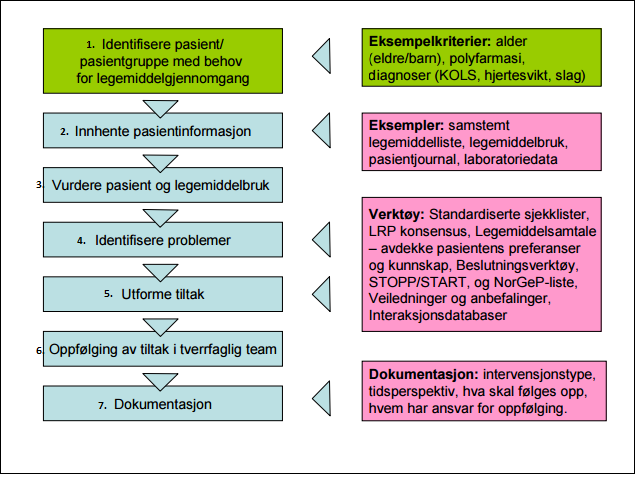
\includegraphics{images/skjematisk_fremgangsmaate_lmg.png}
\caption{Skjematisk fremgangsmåte for legemiddelgjennomgang}
\label{fig:lmgfremgangsmate}
\end{figure}

Hvert steg av fremgangsmåten er viktig for pasientens legemiddelbruk sikkerhet. Under ønsker vi å se nærmere på hva stegene innebærer.

\begin{enumerate}
\item \textbf{Identifisere pasient/pasientgruppe med behov for legemiddelgjennomgang}\\ 
Identifisering av pasient/pasientgruppen er utslagsgivende for når og hvor ofte det skal gjennomføres legemiddelgjennomgang.
Ved denne fasen vil pasientens alder, sykdomstilstand og behov bli identifisert.
\item 
\textbf{Innhenting av nødvendig pasientinformasjon}\\ 
Dette er et viktig grunnlag for aktuelle diagnoser og gir indikasjon for legemiddelbehandling. Her må det være gjennomført grundig og bred klinisk undersøkelse med supplerende informasjon. 

\begin{description}
\item[Legemiddelsamstemming]
Informasjon om den enkelte pasients legemiddelbruk er en viktig forutsetning for en meningsfull legemiddelgjennomgang.
Før en legemiddelgjennomgang utføres må det hentes inn en oppdatert oversikt over de legemiddlene en pasient bruker. Dette kalles en samstemt legemiddelliste og skal inkludere informasjon fra flest mulig av de aktuelle og tilgjengelige kildene. Dersom det er avvik mellom de forskjellige informasjonskildene, må dette komme frem i listen og avklares før eller under en legemiddelgjennomgang. Denne listen skal følge med pasienten ved et eventuelt omsorgsskifte. Prosedyrer for legemiddelsamstemming skal etableres ved de lokale institusjoner.
\end{description}

\begin{description}
\item[Kommunikasjon med pasient/pårørende] 
En annen informasjonskilde som er viktig for legemiddelgjennomgang er pasientens egen forståelse og motivasjon. Dette er for å sikre best mulig etterlevelse av legemiddelbehandlingen. For enkelte pasientgrupper er det viktig med dialog med pårørende. For pasienten kan informasjonen som blir utvekslet under en legemiddelgjennomgang være en mulig til å kunne medvirke i egen behandling. Dette kan bidra til riktigere bruk og gi pasienten mulig til å selv kjenne igjen legemiddelrelaterte problemer.
\end{description}

Det finnes også annen informasjon som er viktig for legemiddelgjennomgangen. Informasjon som bruk av naturmidler, kosttilskudd og ikke-reseptbelagte legemiddler bør innhentes. Det kan også være aktuelt å innhente informasjon om tidligere allergier og signifikante bivirkninger av legemidlene som skal brukes/har vært brukt.

\item \textbf{Vurdere pasient og legemiddelbruk}\\
For å støtte legemiddelvalg med bakgrunn i legemiddelgjennomgang må det benyttes beslutningsstøtteverktøy, sjekklister, interaksjonsdatabaser og liknende.\\
Under er ei typisk liste over hvilken informasjon som trengs om pasient og legemiddelbruk:
\begin{itemize}
\item Hvilke indikasjoner har pasienten?
\item Får pasienten behandling for alle behandlingstrengende indikasjoner?
\item Har pasienten indikasjon for alle legemidlene som er forskrevet?
\item Kan noen av indikasjonene skyldes bivirkninger og/eller interaksjoner forårsaket av andre legemidler?
\item Er behandlingen i samsvar med behandlingsretningslinjer?
\item Avklar pasientens evne og vilje til å ta legemidler og ev. håndtere disse selv 
\end{itemize}

\item 
\textbf{Identifisere legemiddelrelaterte problemer}\\
 Med stadig flere legemidler og flere pasienter som bruker legemidler, gjerne flere samtidig, øker risiko for bivirkninger og legemiddelinteraksjoner, og gjennomføring av medisineringen blir vanskeligere. \citep{DNL_klassifisering_av_legemiddelrelaterte_problemer} \\

Under er legemiddelrelaterte problemer tematisk satt opp. Ut fra spørsmålene under hvert område vurderes det om pasienten har et aktuelt eller et potensielt legemiddelrelatert problem.\citep{Helsedirektoratet_veileder_LMG}

\begin{description}
\item[Legemiddelvalg:]
    \begin{itemize}
    \item[]
    \item Er det fortsatt indikasjon for legemidlet?
  \item Har pasienten tilstrekkelig effekt av legemidlet?
  \item Bruker pasient kurlegemiddel
  \item Mangler pasienten legemiddel for diagnoser/ tilstand? \textit{For eksempel: Jern, vitamin B12, folsyre, protonpumpehemmere,analgetika, antidepressiva og antikoagulantia}
  \item Er legemidlet hensiktsmessig for denne pasienten? \textit{ Bruk beslutningsstøtte-verktøy og oppslagsverktøy. Kontroller at pasienten ikke er satt på legemiddel som er registrert under CAVE/legemiddel-følsomhet.}
  \item Har pasienten ubehandlet indikasjon/tilstand (manglerlegemiddel)?
\end{itemize}

\item[Dosering:]
\begin{itemize}
\item[]
\item Er dosen, doserings-tidspunkt og administrasjon i samsvar med pasientens nåværende situasjon?
\item Kontroller om legemiddel og doser er tilpasset den enkelte pasient med \textit{hensyn til bl.a. nyrefunksjon, leverfunksjon, kontraindikasjoner og andre sykdommer.}
\end{itemize}

\item[Bivirkning:]
\begin{itemize}
\item[]
\item Tolererer pasienten legemidlet? 
\item Har pasienten bivirkninger?
\item Er pasienten/ pårørende kjent med hva hun/han selv må være oppmerksom på når det gjelder administrering, kost, alkohol, interaksjoner med ikke-registrerte legemidler (naturpreparater).
\item Kontroller om legemiddel kan være årsak til bivirkninger, symptom eller forandrede labverdier
\end{itemize}

\item[Interaksjon:]
\begin{itemize}
\item[]
\item Er det interaksjoner av klinisk betydning mellom legemiddellegemiddel eller mellom legemiddel-sykdom eller legemiddel-mat/helsekost og liknende?
\end{itemize}

\item[Avvikende legemiddelbruk:]
\begin{itemize}
\item[]
\item Håndterer og bruker pasienten legemiddelet slik angitt i kurve/journal, og dersom ikke – hvordan gjør/bruker pasienten det? 
\item Er det praktiske håndteringsproblem? 
\small
\begin{itemize}
\item Kontroller om det er behov for knusing av tabletter/ åpning av kapsler pga. svelgeproblemer/ sonde.
\item Hvis pasienten bruker øyedråper, inhalatorer eller lignende 
\item Sjekk teknikk
\end{itemize}
\end{itemize}

\item[Manglende monitorering:]
\begin{itemize}
\item[]
\item Håndterer og bruker pasienten legemiddelet slik angitt i kurve/journal, og dersom ikke – hvordan gjør/bruker pasienten det? 
\item Er det praktiske håndteringsproblem? 
\small
\begin{itemize}
\item Kontroller om det er behov for knusing av tabletter/ åpning av kapsler pga. svelgeproblemer/ sonde.
\item Hvis pasienten bruker øyedråper, inhalatorer eller lignende 
\item Sjekk teknikk
\end{itemize}
\end{itemize}

\item[Andre problemstillinger:]
\begin{itemize}
\item[]
\begin{itemize}
\item[]
\item Er det eventuelle andre momenter å diskutere når det gjelder legemiddelregimet? 
\item Avvik i legemiddelliste.
\end{itemize}
\end{itemize}
\end{description}

\item \textbf{Utforme forslag til tiltak}\\
En legemiddelgjennomgang kan føre frem synlige behov for justing av legemiddelterapien.Endringene/tiltakene utformes med bakgrunn i de avdekkede legemiddelrelaterte problemene. Hvis det skulle oppstå uenigheter i det tverrfaglige teamet er det legen som tar den endelige avgjørelsen.

\item \textbf{Oppfølging av foreslåtte tiltak i tverrfaglige team
}\\
I et tverrfaglig team vil forskjellig helsepersonell ha forskjellige roller, og det er opp til det enkelte helseforetak å organisere seg på best mulig måte. Uavhengig av denne organiseringen er det behandlende lege som tar den endelige avgjørelsen. 

Oppgavene som er knyttet til legemiddelgjennomgangen er avhengig av behandlingstedet, men under er en liste over særlige aktuelle tema:

\begin{itemize}
\item Gi faglig rådgivning om legemiddelbruk: blant annet interaksjoner, alternative legemidler, dosering, potensielle bivikrninger
\item Koordinere legemiddelgjennomgangen
\item Kartlegge pasientens mentale funksjon, bla. i dagliglivets aktiviteter. Dette er særlig aktuelt ved institusjoner og i hjemmebasert omsorg
\item Registrere pasientens evne til å etterleve legemiddlebehandlingen
\item Registere om pasienten trenger bistand til endringer
\item Observere pasienten
\item Generell observasjon av pasient i etterkant av legemiddelendringer
\item Dokumentere/melde dette tilbake til behandlende lege
\item Vurdere ikke-medikamentell behandling
\end{itemize}
Ved foretak hvor tverrfaglige team ikke lar seg enkelt etableres, vil det være naturlig for behandlende lege og forhøre seg med andre leger hvis pasientens legemiddelbilde er komplisert.

\item \textbf{Dokumentasjon av gjennomgangen} \\
Dokumentasjon av legemiddelgjennomgangen skal inneholde:
\begin{itemize}
\item Hvilke legemiddelrelaterte problemer er avdekket
\item Hva krever tiltak og/eller oppfølging
\item Til hvilket tidspunkt skal tiltakene utføres, og av hvem
\end{itemize}
Dersom det utføres ekstra utredning i forbindelse med gjennomgangen (litteratursøk, omfattende interaksjonsøk og liknende) må det vurderes om dette skal registreres i elektronisk pasientjournal.
\end{enumerate}




%\begin{itemize}
%\item Hva er legemiddelgjennomgang.\\
%Sikre bruken av legemiddler og forebygge skader. \\
%Se kapittel 2.2 i [3], her er det mye som kan brukes.
%\item Hvorfor gjennomføres legemiddelgjennomgang.

%\item Hvordan utføres en legemiddelgjennomgang i dag.
%\item Kan nevne LMS (Legemiddelsamstemning) og LIB (Legemiddler i bruk). \\
%Legemiddelgjennomgang krever at en samstemt legemiddel liste er tilgjengelig.
%\end{itemize}
\section{Legemiddelgjennomgang i Midt-Norge}
Prosessen med å ha tjenester som kan sjekke legemiddeldoseringer og legemiddelrelaterte problemer hos pasienter i spesialhelsetjenesten startet for tjue år siden i Midt-Norge. Kliniske farmasøyter ble sendt ut på post for å utfylle noe av jobben for sykepleiere og leger. I Midt-Norge fungerer kliniske farmasøyter som en tjeneste som kan benyttes på forskjellige poster hvor det er behov for legemiddelsamtstemming, legemiddelgjennomgang og andre legemiddelhåndteringer. 

\subsection{IMM-modellen}
På 2000-tallet ble \gls{imm} utviklet ved Queens University of Belfast i Nord-Irland. Dette er en modell for utøving av klinisk farmasi. Målet med modellen er å oppnå maksimal helse gjennom optimal bruk av legemidler.  \gls{imm} beskriver en sømløs prosess og integrerer behandlingsnivåene i hverandre i tillegg til
å integrere farmasøyten i det tverrfaglige behandlingsteamet. 

Det er systematisk måte å jobbe på for å :
\begin{itemize}
\item å kvalitetessikre pasientens legemiddelliste
\item å individualisere og optimalisere legemiddelbehandlingen for pasienter
\item å sikre informasjonsoverføring til andre omsorgsnivåer (sykehjem, fastlege, hjemmesykepleier)
\item å involverer pasienten til å forstå legemiddelbehandlingen
\end{itemize}
I Lund i Sverige ble IMM-modellen videreutviklet og tilpasset svenske forhold og ble dermed til \gls{limm}. \gls{limm} har strukturerte og forskningsbaserte prosedyrer og verktøy inkludert faglige dokumenter til å vurdere den enkelte pasientens legemiddelbehandling. \gls{limm} inneholder også spesifikke kompetansekrav og standardiserte opplæringsprosedyrer. 

I 2010 ble \gls{limm} utviklet i Midt-Norge med utgangspunkt i den svenske \gls{limm}. \gls{imm} i Midt-Norge har som mål å forbedre legemiddelbehandlingen til den enkelte pasienten og har fokus på tverrfaglig samarbeid. Den kliniske farmasøyten har som oppgave å identifisere, løse og forebygge legemiddelrelaterte problemer og kommer med forslag og innspill til legen for å kvalitetssikre legemiddelbehandlingen. Modellen involverer moduler til bruk ved innleggelse, under sykehusopphold og ved utskrivning. I figur \ref{fig:imm}  blir det illustrert hva som gjøres under hver hendelse, hvor legemiddelgjennomgang er en del av sykehusoppholdet.
\\\citep{IMM_i_midtnorge}

\begin{figure}[H]
\centering
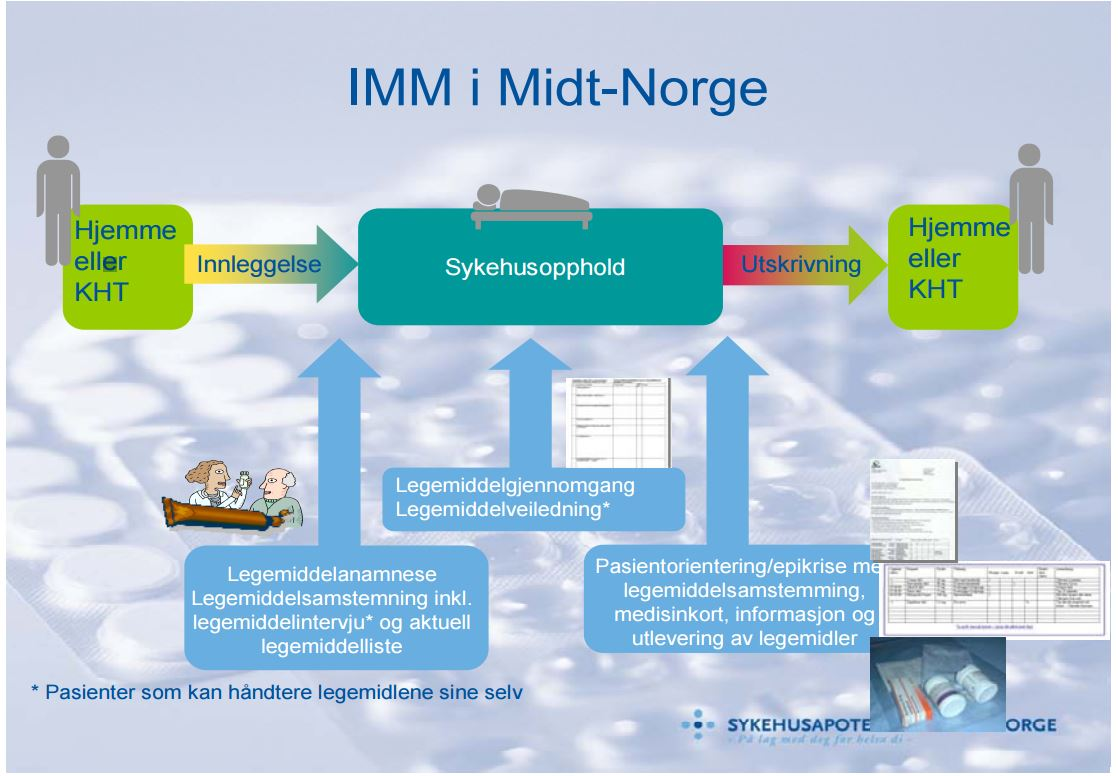
\includegraphics[width= 12cm]{images/IMM_I_MIDT_NORGE.JPG}
\caption{IMM i Midt-Norge}
\label{fig:imm}
\end{figure}

Da IMM-modellen ble tatt i bruk skapte dette en interesse for NTNU. Modellen har strukturerte og forskningsbaserte prosedyrer, og dette førte til et IMM-kurs på NTNU. Sykehusapotekene i Midt-Norge og Det medisinske fakultet ved NTNU fikk midler til å utvikle et farmasøytisk videre- og etterutdanningstilbud. Målet med kurset er at farmasøyter skal kunne fungere som legemiddelspesialister i tverrfaglige team for å oppnå riktig legemiddelbruk for pasientene, og jobbe med klinisk farmasi i henhold til IMM-modellen.  \citep{IMM_MODELLEN_TIL_NORGE} \citep{MDV6000}
